\section{Sprint 3 : Maintenance préventive}

\subsection{Introduction}

Après la structuration du parc industriel et de la documentation technique, ce troisième Sprint est consacré à la maintenance préventive. Il porte sur la gestion des plans, des tâches et des listes de contrôle, sur la planification des occurrences ainsi que sur le cycle de validation des interventions.

La maintenance préventive constitue l'un des axes centraux de la plateforme. Elle permet de transformer les plans actuellement répartis entre plusieurs documents en opérations planifiées, affectées et suivies dans un système commun. Elle vise à réduire les défaillances imprévues, à organiser la charge de travail et à conserver un historique des contrôles réalisés sur chaque équipement.

Ce chapitre présente les objectifs et le Sprint Backlog, puis la conception du flux préventif. Il décrit ensuite les fonctionnalités réalisées, notamment la planification des échéances, l'exécution des listes de contrôle et la validation des interventions, avant de présenter les tests de validation.

\subsection{Objectifs du Sprint}

L'objectif principal de ce Sprint est de permettre à l'entreprise de planifier, d'exécuter et de suivre ses opérations de maintenance préventive.

Les objectifs spécifiques sont les suivants :

\begin{itemize}
    \item gérer les plans de maintenance préventive et leur cycle de vie ;
    \item associer un plan à une machine ou à un module ;
    \item définir les tâches, les fréquences et les unités de planification ;
    \item gérer les listes de contrôle associées aux plans ;
    \item planifier la première occurrence d'un plan ;
    \item générer les échéances suivantes selon la périodicité définie ;
    \item permettre à l'opérateur d'exécuter et de soumettre une intervention ;
    \item permettre au technicien ou à l'administrateur de valider l'intervention ;
    \item replanifier une occurrence en cas de contrainte opérationnelle ;
    \item consulter l'état préventif et l'historique d'une machine.
\end{itemize}

À la fin du Sprint, l'administrateur doit pouvoir structurer les plans préventifs, l'opérateur doit pouvoir exécuter les listes de contrôle qui lui sont affectées et le technicien doit pouvoir valider les interventions réalisées.

\subsection{Sprint Backlog}

Le tableau~\ref{tab:sprint3-backlog} recense les tâches planifiées pour ce Sprint.

{\small
\setlength{\tabcolsep}{5pt}
\begin{longtable}{|p{1cm}|p{10.3cm}|p{1.5cm}|p{1.4cm}|}
\caption{Sprint Backlog du Sprint 3}
\label{tab:sprint3-backlog}\\
\hline
\textbf{ID} & \textbf{Tâche} & \textbf{Priorité} & \textbf{Statut} \\
\hline
\endfirsthead

\hline
\textbf{ID} & \textbf{Tâche} & \textbf{Priorité} & \textbf{Statut} \\
\hline
\endhead

S3-01 &
Développer le modèle et le cycle de vie des plans préventifs. &
Haute & Réalisé \\
\hline

S3-02 &
Gérer les tâches et les listes de contrôle des plans. &
Haute & Réalisé \\
\hline

S3-03 &
Synchroniser les listes de contrôle avec les plans existants. &
Moyenne & Réalisé \\
\hline

S3-04 &
Planifier la première occurrence d'un plan. &
Haute & Réalisé \\
\hline

S3-05 &
Développer l'exécution et la soumission des interventions par l'opérateur. &
Haute & Réalisé \\
\hline

S3-06 &
Mettre en place la validation par un technicien ou un administrateur. &
Haute & Réalisé \\
\hline

S3-07 &
Générer automatiquement la prochaine échéance après validation. &
Haute & Réalisé \\
\hline

S3-08 &
Permettre la replanification d'une occurrence préventive. &
Moyenne & Réalisé \\
\hline

S3-09 &
Développer la consultation de l'état préventif d'une machine. &
Moyenne & Réalisé \\
\hline

S3-10 &
Vérifier le flux préventif par des tests et un audit de planification. &
Haute & Réalisé \\
\hline

\end{longtable}}

\subsection{User Stories du Sprint}

Les fonctionnalités de ce Sprint reprennent les User Stories US05 et US06 du Product Backlog :

\begin{itemize}
    \item \textbf{US05 :} en tant qu'administrateur, je souhaite gérer les plans et les tâches préventives afin de planifier les opérations de maintenance ;
    \item \textbf{US06 :} en tant qu'opérateur, je souhaite exécuter et soumettre les listes de contrôle afin d'assurer le suivi des opérations préventives.
\end{itemize}

\subsection{Conception du Sprint}

\subsubsection{Diagramme des cas d'utilisation}

Le diagramme de la figure~\ref{fig:usecase-preventive} présente les cas d'utilisation du flux préventif. L'administrateur crée et structure les plans et leurs listes de contrôle ; le technicien consulte les plans, valide les interventions et peut replanifier une occurrence ; l'opérateur exécute et soumet les interventions qui lui sont affectées. Un acteur système, le planificateur automatique, prend en charge la génération des échéances suivantes.

\begin{figure}[H]
    \centering
    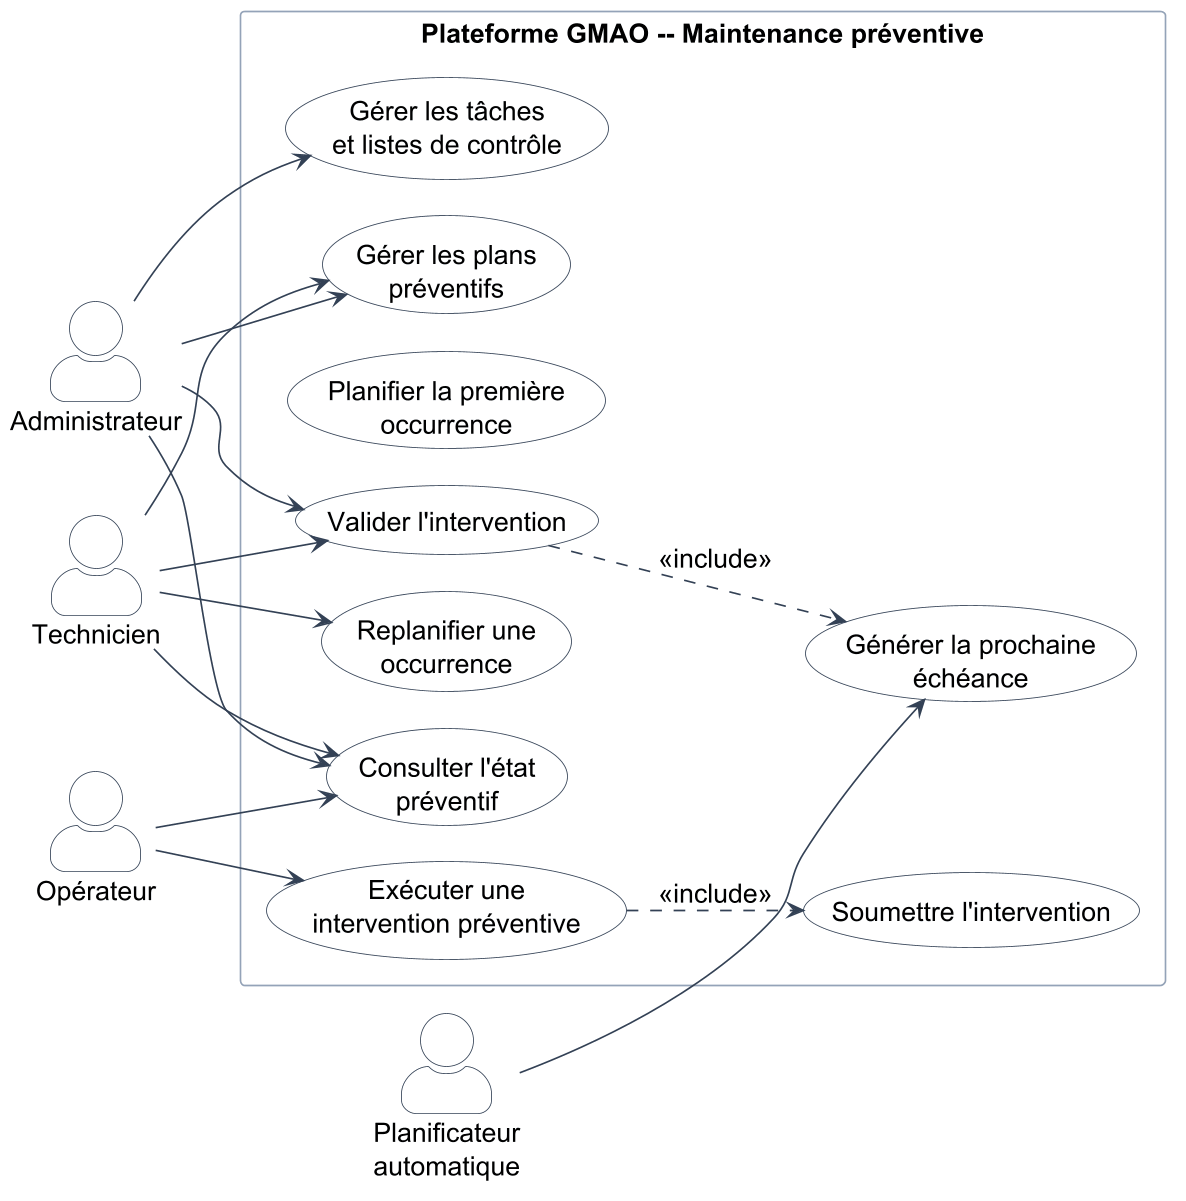
\includegraphics[width=0.92\textwidth,height=0.72\textheight,keepaspectratio]{figures/usecase-preventive.png}
    \caption{Diagramme des cas d'utilisation du Sprint 3}
    \label{fig:usecase-preventive}
\end{figure}

L'exécution inclut la soumission de l'intervention, et la validation inclut la génération de la prochaine échéance : une occurrence n'est donc considérée comme réalisée qu'après la validation d'un technicien ou d'un administrateur.

\subsubsection{Tâches et listes de contrôle}

Chaque plan regroupe les tâches à exécuter lors de l'intervention. Une tâche peut correspondre à un contrôle, un nettoyage, une lubrification, un graissage ou un remplacement périodique.

Les tâches sont organisées en listes de contrôle afin de guider l'opérateur pendant l'intervention. Chaque élément comporte une description, un ordre d'exécution et, lorsque nécessaire, des consignes ou des références aux documents techniques.

La synchronisation des listes de contrôle permet de reprendre les tâches définies dans les plans importés et de les structurer dans la plateforme. L'opérateur peut ainsi cocher les opérations réalisées et renseigner les observations ou anomalies constatées.
\subsubsection{Planification des occurrences}

À l'activation d'un plan, la première occurrence est planifiée selon la date de début et la fréquence définies. L'opérateur affecté retrouve cette occurrence dans son calendrier et dans son espace de travail.

Lorsqu'une intervention est validée, le service de planification calcule la prochaine échéance à partir de la fréquence du plan. Cette génération automatique évite la ressaisie des opérations périodiques et limite les oublis.

Le tableau~\ref{tab:unites-frequence} présente les principales unités de planification prises en charge.

\begin{table}[H]
\centering
\caption{Unités de planification préventive}
\label{tab:unites-frequence}
\small
\begin{tabularx}{0.8\textwidth}{|p{3.8cm}|X|}
\hline
\textbf{Unité} & \textbf{Usage typique} \\
\hline
Jour & Contrôles quotidiens ou fréquents \\
\hline
Semaine & Contrôles hebdomadaires \\
\hline
Mois & Opérations mensuelles \\
\hline
Trimestre & Contrôles périodiques \\
\hline
Semestre & Opérations semestrielles \\
\hline
Année & Remplacements ou contrôles annuels \\
\hline
\end{tabularx}
\end{table}

\subsubsection{Exécution et soumission par l'opérateur}

L'opérateur consulte les occurrences préventives qui lui sont affectées. Il ouvre l'intervention, parcourt la liste de contrôle et renseigne les résultats de chaque tâche.

Il peut ajouter des observations, signaler une anomalie détectée pendant le contrôle et joindre les informations utiles. Une fois les tâches renseignées, il soumet l'intervention pour validation.

L'intervention reste dans un état en attente de validation. Elle ne génère pas encore l'échéance suivante, ce qui garantit qu'un contrôle non validé ne soit pas considéré comme réalisé.

Les opérations relevant de la maintenance corrective restent traitées dans le Sprint suivant. Le présent Sprint se limite aux interventions issues d'un plan préventif.
\subsubsection{Validation et génération de la prochaine échéance}

Le technicien ou l'administrateur examine l'intervention soumise, les tâches effectuées et les observations de l'opérateur. Il peut valider l'intervention ou la rejeter en précisant le motif.

Après validation, le système marque l'occurrence comme réalisée puis crée la prochaine échéance en appliquant la périodicité du plan. La date, l'opérateur affecté et la liste de contrôle sont repris pour la nouvelle occurrence.

Le système conserve la trace de la validation, de son auteur et de sa date. Cette traçabilité permet de vérifier le respect du plan et d'alimenter les indicateurs de conformité de la maintenance préventive.

\begin{figure}[H]
    \centering
    \IfFileExists{figures/sprint3-preventive-validation.png}{%
        \includegraphics[width=0.95\textwidth,height=0.82\textheight,keepaspectratio]{figures/sprint3-preventive-validation.png}%
    }{%
        \fbox{\parbox[c][7cm][c]{0.92\textwidth}{\centering\itshape Capture d'écran à insérer\\[2mm]\texttt{figures/sprint3-preventive-validation.png}}}%
    }
    \caption{Validation d'une intervention préventive}
    \label{fig:sprint3-preventive-validation}
\end{figure}
\subsubsection{Replanification et suivi de l'état préventif}

Lorsqu'une occurrence ne peut pas être réalisée à la date prévue, un technicien ou un administrateur peut la replanifier. L'opération conserve le lien avec le plan d'origine et reporte la nouvelle date dans le calendrier.

La consultation de l'état préventif d'une machine regroupe les occurrences planifiées, en attente de validation, réalisées en retard ou rejetées. Cette vue permet d'identifier les plans nécessitant une attention particulière.

Le calendrier préventif présente les interventions à venir et facilite l'organisation des équipes. Il est alimenté automatiquement par les échéances générées après validation.

Afin de contrôler la cohérence des dates et des occurrences, un audit de planification a également été mis en place. Il vérifie les occurrences en attente, les dates dépassées et les échéances successives.
\subsubsection{Diagramme d'activités du flux préventif}

Le flux préventif suit une logique de validation avant la génération de l'échéance suivante. Une intervention soumise par l'opérateur n'est considérée comme réalisée qu'après la validation d'un technicien ou d'un administrateur.

Le flux commence par la création du plan et son association à une machine ou à un module, puis par la définition des tâches, de la fréquence et de l'unité de planification. La première occurrence est ensuite planifiée et affectée à un opérateur. Après exécution et soumission, le contrôle de conformité détermine la suite : la validation déclenche la génération de la prochaine échéance, tandis qu'un refus impose une correction et une nouvelle exécution des tâches.

La figure~\ref{fig:activite-preventive} présente ce déroulement.

\begin{figure}[H]
    \centering
    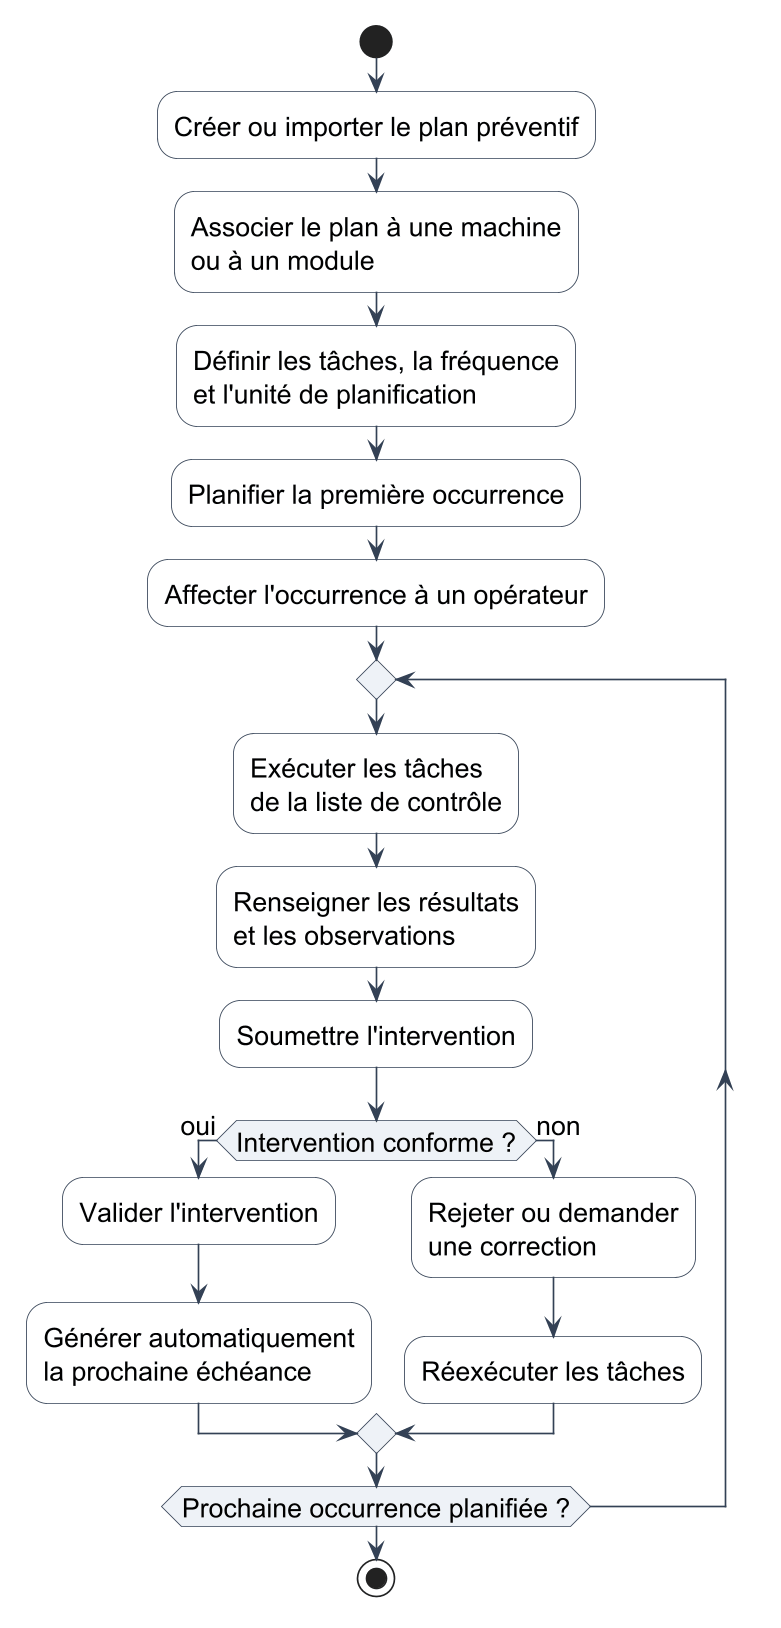
\includegraphics[width=0.7\textwidth,height=0.84\textheight,keepaspectratio]{figures/activity-preventive.png}
    \caption{Diagramme d'activités du flux de maintenance préventive}
    \label{fig:activite-preventive}
\end{figure}

\subsubsection{Diagramme d'états d'un plan préventif}

Un plan de maintenance possède un cycle de vie contrôlé. Il est d'abord créé à l'état de brouillon, puis activé pour permettre la planification des occurrences. Il peut être suspendu, repris, marqué comme terminé ou archivé selon les décisions de l'administrateur.

\begin{figure}[H]
    \centering
    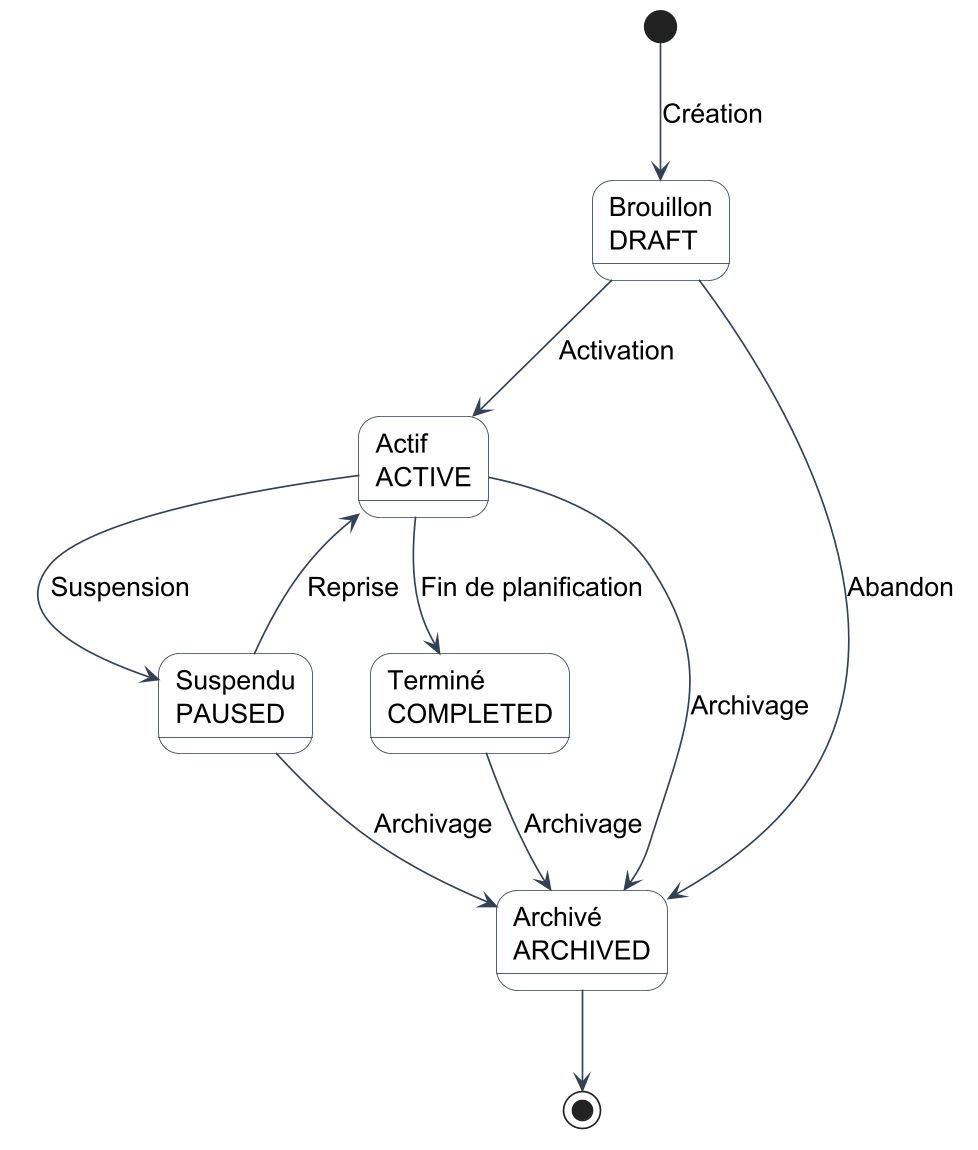
\includegraphics[width=0.78\textwidth,height=0.78\textheight,keepaspectratio]{figures/state-maintenance-plan.png}
    \caption{Diagramme d'états d'un plan de maintenance préventive}
    \label{fig:state-maintenance-plan}
\end{figure}

Les transitions traduisent les décisions de gestion : l'activation autorise la planification, la suspension interrompt temporairement la génération des occurrences et la reprise la rétablit. L'archivage clôt le cycle de vie du plan, quel que soit son état précédent, sans supprimer l'historique des interventions associées.

\subsubsection{Diagramme de séquence de la validation préventive}

La figure~\ref{fig:sequence-preventive} présente les échanges entre l'opérateur, l'interface, l'API et le service de planification lors de la validation d'une intervention.

\begin{figure}[H]
    \centering
    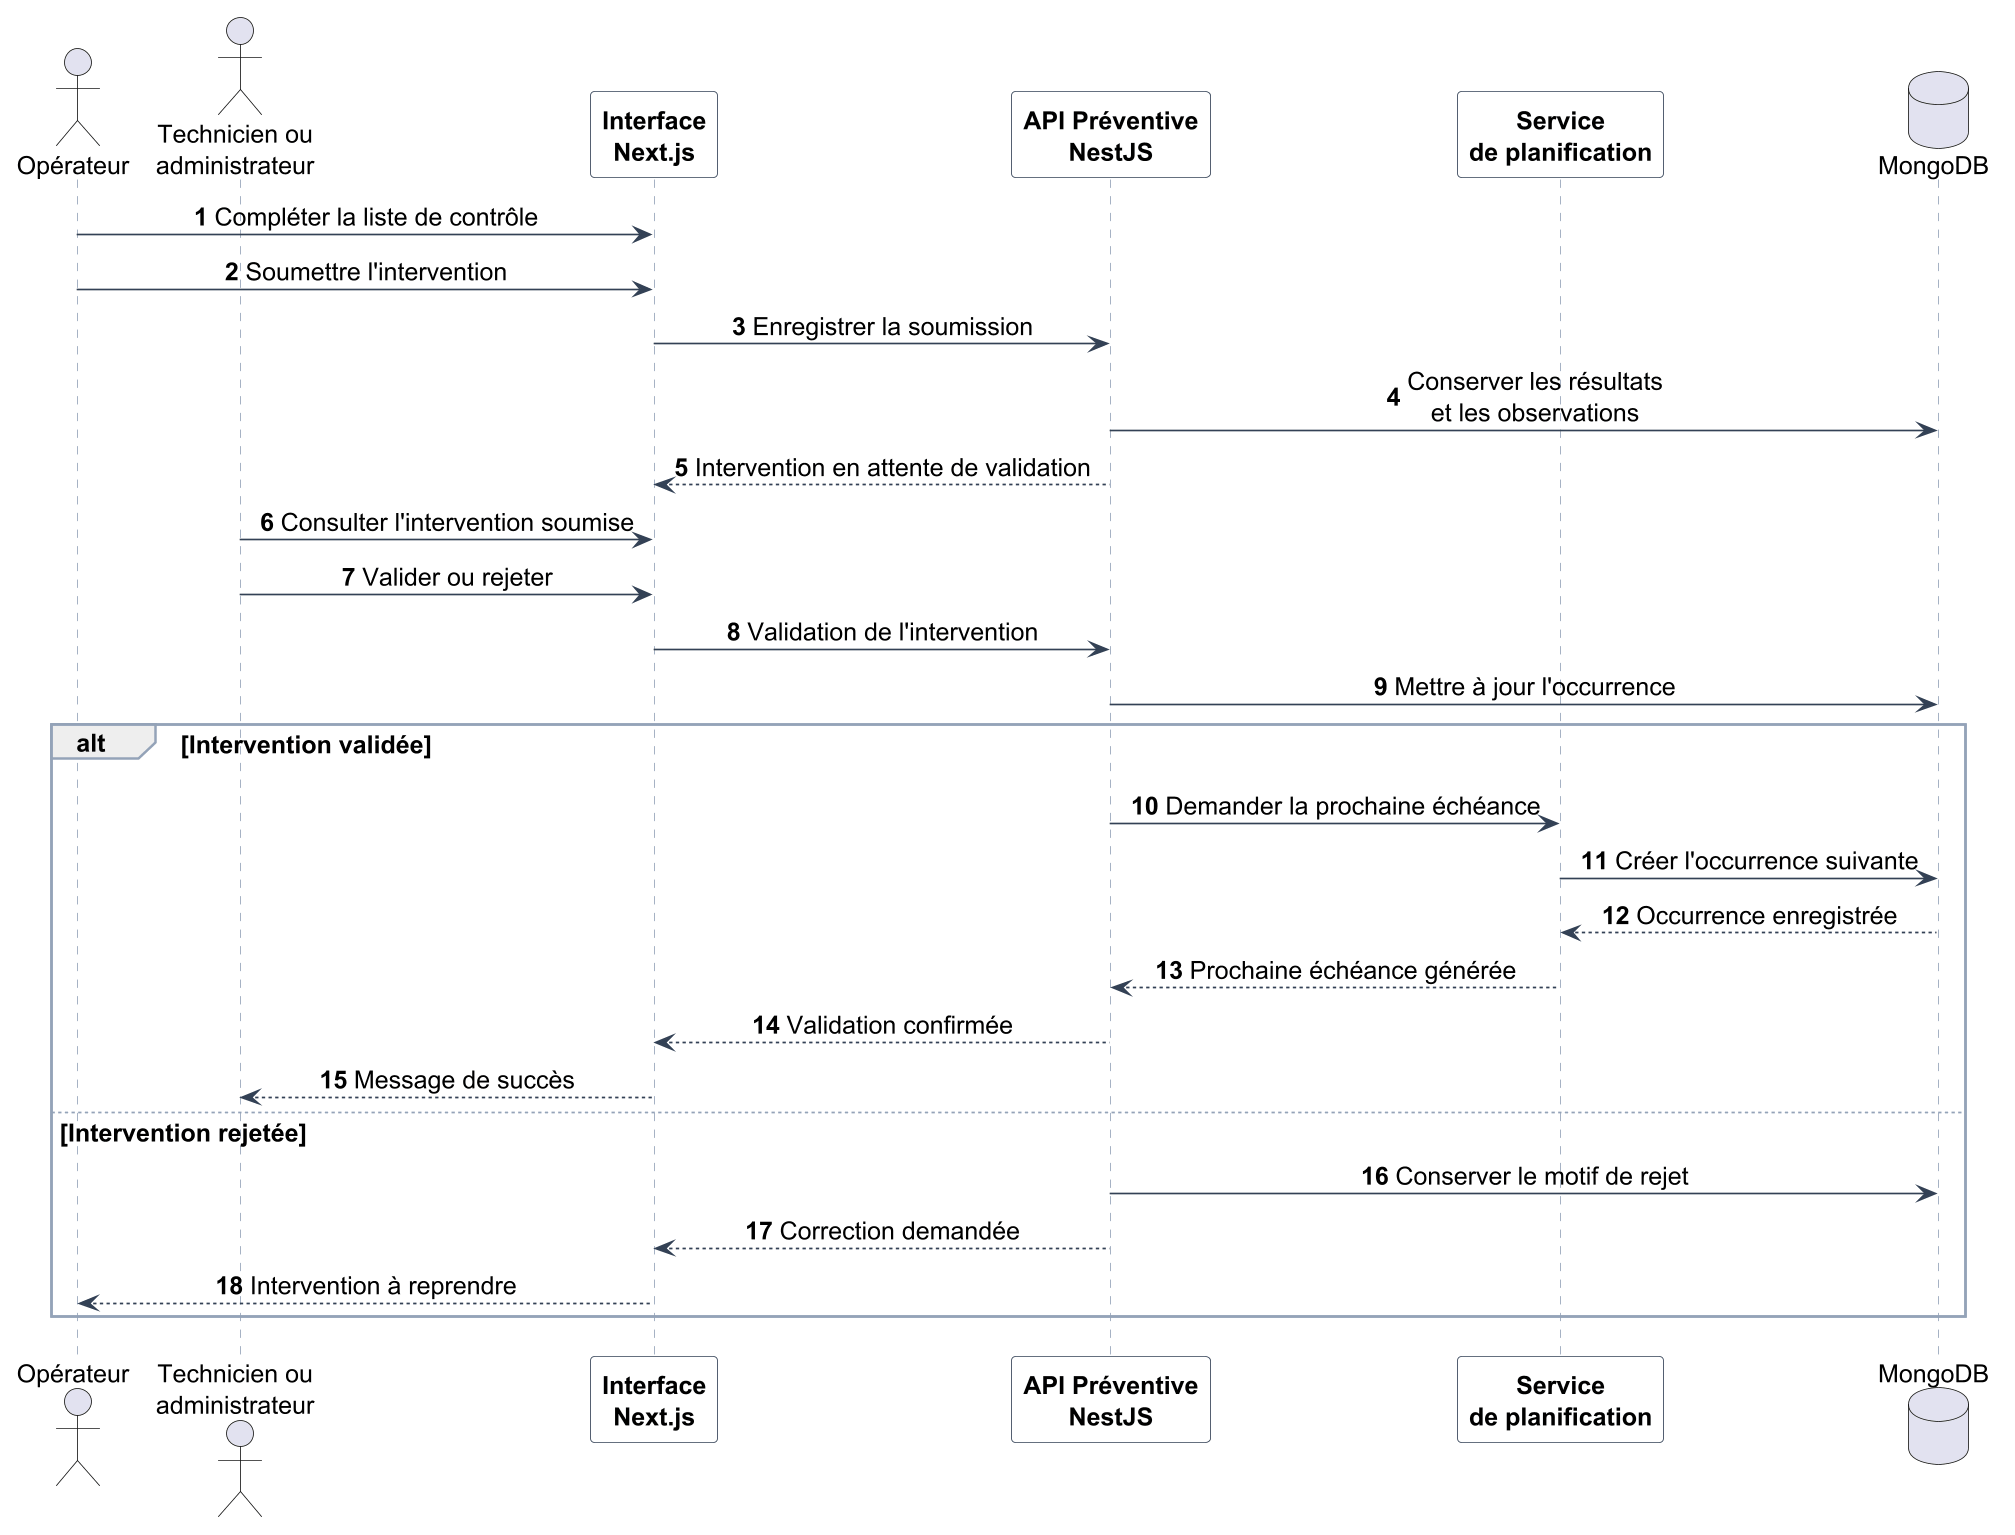
\includegraphics[width=\textwidth,height=0.80\textheight,keepaspectratio]{figures/sequence-preventive-validation.png}
    \caption{Diagramme de séquence de la validation d'une intervention préventive}
    \label{fig:sequence-preventive}
\end{figure}

Lors de l'ouverture de l'occurrence, l'API charge le plan et sa liste de contrôle depuis la base et transmet les tâches à l'interface. L'opérateur renseigne les résultats, puis soumet l'intervention : celle-ci est enregistrée dans un état d'attente de validation. La validation est ensuite traitée par l'API, qui contrôle le rôle de l'utilisateur et la conformité de l'intervention. En cas de conformité, l'occurrence est marquée comme validée et le service de planification crée l'échéance suivante ; dans le cas contraire, l'occurrence reste en attente et une correction est demandée.

\subsection{Réalisation}

\subsubsection{Gestion des plans préventifs}

Le module des plans permet à l'administrateur de créer un plan, de le rattacher à une machine ou à un module et de définir sa périodicité. Chaque plan précise le type de maintenance, la fréquence, l'unité de fréquence et les tâches à réaliser.

Un plan peut être créé manuellement ou importé à partir des référentiels existants. L'importation facilite la reprise des plans de tressage, de découpe, d'enroulage et de bobinage sans ressaisie complète.

Le cycle de vie du plan est contrôlé : un plan suspendu ne génère pas de nouvelle occurrence, tandis qu'un plan archivé reste consultable pour l'historique mais n'est plus planifié.

\begin{figure}[H]
    \centering
    \IfFileExists{figures/sprint3-plans-list.png}{%
        \includegraphics[width=0.95\textwidth,height=0.82\textheight,keepaspectratio]{figures/sprint3-plans-list.png}%
    }{%
        \fbox{\parbox[c][7cm][c]{0.92\textwidth}{\centering\itshape Capture d'écran à insérer\\[2mm]\texttt{figures/sprint3-plans-list.png}}}%
    }
    \caption{Liste des plans de maintenance préventive}
    \label{fig:sprint3-plans-list}
\end{figure}

\subsection{Tests et validation}

Le tableau~\ref{tab:tests-sprint3} présente une synthèse des scénarios vérifiés pour ce Sprint.

{\footnotesize
\setlength{\tabcolsep}{4pt}
\begin{longtable}{|p{0.9cm}|>{\raggedright\arraybackslash}p{7cm}|>{\raggedright\arraybackslash}p{4.7cm}|}
\caption{Scénarios de test du Sprint 3}
\label{tab:tests-sprint3}\\
\hline
\textbf{ID} & \textbf{Scénario} & \textbf{Résultat attendu} \\
\hline
\endfirsthead

\hline
\textbf{ID} & \textbf{Scénario} & \textbf{Résultat attendu} \\
\hline
\endhead

T3-01 &
Création d'un plan préventif avec une fréquence mensuelle &
Plan enregistré et première occurrence planifiée \\
\hline

T3-02 &
Activation d'un plan suspendu &
Nouvelles occurrences autorisées \\
\hline

T3-03 &
Suspension d'un plan &
Aucune nouvelle occurrence générée \\
\hline

T3-04 &
Importation d'un plan existant &
Tâches et fréquences reprises correctement \\
\hline

T3-05 &
Exécution d'une occurrence par l'opérateur &
Liste de contrôle disponible et résultats enregistrés \\
\hline

T3-06 &
Soumission d'une intervention incomplète &
Validation refusée et tâches manquantes signalées \\
\hline

T3-07 &
Validation d'une intervention conforme &
Prochaine occurrence générée automatiquement \\
\hline

T3-08 &
Rejet d'une intervention &
Intervention conservée en correction sans nouvelle échéance \\
\hline

T3-09 &
Replanification d'une occurrence &
Nouvelle date enregistrée et calendrier mis à jour \\
\hline

T3-10 &
Consultation de l'état préventif d'une machine &
Occurrences et statuts affichés correctement \\
\hline

T3-11 &
Audit de planification &
Aucune incohérence de dates ou d'échéances \\
\hline

\end{longtable}}

Les tests ont confirmé le respect du cycle de validation : une intervention n'est considérée comme réalisée qu'après validation, et la prochaine échéance n'est créée qu'à partir d'une intervention conforme. Les tests automatisés couvrent notamment la logique des plans, des listes de contrôle et de la génération des échéances.

\subsection{Revue du Sprint et conclusion}

Lors de la revue, la création des plans, la préparation des listes de contrôle, l'exécution par l'opérateur et la validation par le technicien ont été présentées.

Les principaux résultats du Sprint sont les suivants :

\begin{itemize}
    \item centralisation des plans de maintenance préventive ;
    \item transformation des plans existants en tâches et listes de contrôle ;
    \item planification de la première occurrence et génération automatique des échéances ;
    \item exécution et soumission des interventions par les opérateurs ;
    \item contrôle de la conformité par validation humaine ;
    \item replanification des occurrences et suivi de l'état préventif des machines ;
    \item alimentation du calendrier et des indicateurs de maintenance.
\end{itemize}

La rétrospective a confirmé que ce module apporte une valeur métier importante, puisqu'il structure un processus déjà présent dans l'entreprise tout en améliorant sa traçabilité.

Le Sprint 4 sera consacré à la maintenance corrective et aux ordres de travail.
